% file: no-ot-ab.tex

\documentclass[tikz]{standalone}
\usetikzlibrary{shapes, positioning, arrows.meta, calc, backgrounds, fit}

\newcommand{\ins}[2]{\textsc{Ins}(#1,#2)}
\newcommand{\del}[1]{\textsc{Del}(#1)}

\begin{document}
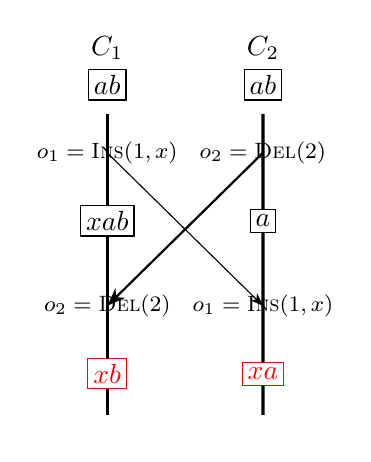
\begin{tikzpicture}[
	timeline/.style = {very thick}, >=Stealth, 
	send/.style = {>=Stealth, ->},
	list/.style = {rectangle, draw, inner sep = 2pt, outer sep = 0pt},
	op/.style = {font = \footnotesize}
  ]
  \node[list, label = {above:{$C_1$}}] (r1) {$ab$}; 
  \node[list, right = 1.50cm of r1, label = {above:{$C_2$}}] (r2) {$ab$};

  \begin{scope}[on background layer]
    \foreach \r/\rbot in {r1/r1bot, r2/r2bot} {
      \node[below = 4.0cm of \r] (\rbot) {};
    }
  \end{scope}

  \draw[send] ($(r1)!0.20!(r1bot)$) node[op] (ins) {$o_1 = \ins{1}{x}$} to ($(r2)!0.65!(r2bot)$) node[op] () {$o_1 = \ins{1}{x}$};
  \draw[send, thick] ($(r2)!0.20!(r2bot)$) node[op] (del) {$o_2 = \del{2}$} to ($(r1)!0.65!(r1bot)$) 
  	node[op] () {$o_2 = \del{2}$};

  \node (r11) [list] at ($(r1)!0.40!(r1bot)$) {$xab$};
  \node (r12) [red, list] at ($(r1)!0.85!(r1bot)$) {$xb$};

  \node (r21) [list] at ($(r2)!0.40!(r2bot)$) {$a$};
  \node (r22) [red, list] at ($(r2)!0.85!(r2bot)$) {$xa$};

  \draw[timeline] ($(r1.south)+(0,-5pt)$) -- (r11) -- (r12) -- (r1bot);
  \draw[timeline] ($(r2.south)+(0,-5pt)$) -- (r21) -- (r22) -- (r2bot);
\end{tikzpicture}
\end{document}

